\documentclass[conference]{IEEEtran}
\usepackage{graphicx}
\usepackage{amsmath}
\usepackage{amsfonts}
\usepackage{amssymb}
\usepackage{cite}
\usepackage{url}
\usepackage{multirow}
\usepackage{float}
\usepackage{mathptmx}
\usepackage{listings}
\usepackage{subcaption}
\usepackage{booktabs}
\usepackage{tikz}
\usetikzlibrary{shapes.geometric, arrows}

\title{Deep Object Pose Estimation Using DOPE and Synthetic Data}

\author{
\IEEEauthorblockN{Yash Wakde}
\IEEEauthorblockA{\textit{Northeastern University} \\
Boston, MA \\
wakde.y@northeastern.edu}
\and
\IEEEauthorblockN{Deepak Ramesh}
\IEEEauthorblockA{\textit{Northeastern University} \\
Boston, MA \\
ramesh.deep@northeastern.edu}
}


\begin{document}

\maketitle

\begin{abstract}
This project explores the application of Deep Object Pose Estimation (DOPE) for estimating the 6-DoF pose of rigid household objects using RGB images. We focus on two YCB objects: the Cracker Box and the Soup Can. Synthetic datasets containing 20,000 images per object were generated using BlenderProc, allowing for robust training without collecting real-world annotations. These datasets enabled the training of a convolutional neural network (CNN) to detect object keypoints and estimate 3D poses through a Perspective-n-Point (PnP) algorithm. We conducted real-time inference using webcam feeds and evaluated DOPE's performance in various lighting conditions. Our findings demonstrate that the DOPE pipeline, trained exclusively on synthetic data, generalizes effectively to real-world scenarios and provides accurate and stable pose estimation suitable for robotic applications. This report covers the methodology in depth, including the architecture of DOPE, data generation pipeline, training process, inference mechanisms, challenges faced, results, and proposed future improvements.
\end{abstract}

\section{Introduction}
Understanding an object's 6-DoF pose—its position and orientation in 3D space—is a critical capability in robotic manipulation, autonomous systems, and augmented reality. Estimating object pose from visual data allows machines to interact intelligently with the physical world. Traditional approaches to 6-DoF object pose estimation rely heavily on depth sensors, hand-crafted features, or large annotated real-world datasets. These methods often involve high costs, limited flexibility, and difficulty generalizing to unseen environments.

With the advent of deep learning, data-driven approaches have emerged as effective alternatives. DOPE (Deep Object Pose Estimation) is one such method, developed to estimate the 6-DoF pose of known rigid objects using only RGB images. It employs a fully convolutional neural network to predict belief maps and affinity fields, which are then used to recover 3D object poses through the PnP algorithm.

This project focuses on implementing the DOPE pipeline using only synthetic data generated via BlenderProc—a procedural data generation framework built upon Blender. We chose two common YCB (Yale-CMU-Berkeley) objects, the Cracker Box and the Soup Can, and generated over 20,000 synthetic images per object, complete with keypoint annotations and camera intrinsics. The generated data was used to train the DOPE CNN from scratch. Inference was performed using both offline images and real-time webcam input, and the system was extended to detect multiple objects simultaneously.

Our motivation is to demonstrate that a fully synthetic pipeline, when paired with an interpretable deep architecture like DOPE, can produce robust pose estimations suitable for deployment in real-world robotic systems. We provide an in-depth analysis of the DOPE network's components, the training procedure, the PnP algorithm, and our synthetic data generation pipeline. We also discuss the challenges encountered, the performance achieved, and potential improvements.

This report is organized as follows: Section II reviews related work in pose estimation. Section III describes the DOPE architecture and mathematical foundations. Section IV details our synthetic data generation pipeline. Section V outlines the training process and hyperparameters. Section VI explains the inference methods used. Section VII presents the results. Section VIII discusses challenges and mitigations. Section IX concludes with future directions.


\section{Related Work}

Object pose estimation has been a fundamental research area in computer vision and robotics, with significant developments spanning both traditional and deep learning-based methods. Early work in this domain primarily relied on hand-crafted features and geometric reasoning. Algorithms like LINEMOD and various template matching approaches were limited in robustness under varying lighting conditions, occlusions, and textureless surfaces.

The introduction of convolutional neural networks (CNNs) revolutionized object detection and pose estimation. Notable deep learning models such as PoseCNN \cite{xiang2018posecnn}, BB8 \cite{rad2017bb8}, and SSD-6D \cite{kehl2017ssd} significantly improved accuracy and generalizability. PoseCNN introduced a segmentation-based method followed by keypoint voting to estimate 6D pose. BB8 used a two-stage architecture to predict object masks and then regress 2D projections of the 3D bounding box corners. SSD-6D extended the Single Shot Detector to simultaneously detect objects and estimate their 3D pose in real time.

A key bottleneck in training deep models was the requirement for large-scale annotated datasets with accurate 6D pose labels. To address this, Tobin et al. introduced domain randomization \cite{tobin2017domain}, a technique where synthetic images are randomized in texture, lighting, and backgrounds to encourage generalization to real-world data. This approach paved the way for simulation-to-reality transfer.

Building upon this, DOPE (Deep Object Pose Estimation) proposed by Tremblay et al. \cite{tremblay2018dope} presented a novel idea: instead of directly regressing pose parameters or bounding boxes, it used belief maps and affinity fields to detect keypoints in a structured and interpretable manner. These heatmaps offered a visual and explainable representation of the detection process, facilitating downstream use of Perspective-n-Point (PnP) solvers for final pose estimation.

The interpretability and modularity of DOPE made it particularly suitable for robotic applications. Moreover, the fact that it can be trained entirely on synthetic data while achieving robust performance in real-world scenarios makes it a cost-effective and scalable solution for 6D pose estimation. This has inspired subsequent works to explore variations of keypoint-based approaches and hybrid architectures involving segmentation, regression, and voting mechanisms.

In summary, our work draws from a rich lineage of research in pose estimation. We leverage the advances of domain-randomized synthetic training, deep keypoint detectors, and classical geometric solvers to implement and analyze a full DOPE pipeline tailored for YCB objects.
The DOPE framework proposed by Tremblay et al. \cite{tremblay2018dope} offers an interpretable, belief-map based approach using synthetic training data. This makes it ideal for robotics applications with controlled object categories.

\section{DOPE Architecture and Working Principle}

DOPE (Deep Object Pose Estimation), is a fully convolutional neural network designed to predict the 6-DoF (Degrees of Freedom) pose of known rigid objects using only RGB input. Unlike traditional bounding-box-based or direct regression-based pose estimation techniques, DOPE generates intermediate spatial representations in the form of belief maps and affinity fields, enabling interpretable and robust pose estimation suitable for robotic applications.

The design philosophy of DOPE stems from the need for robustness, interpretability, and generalization in pose estimation pipelines. Rather than performing direct regression of pose parameters—which can be noisy and sensitive to overfitting—DOPE introduces intermediate supervision via 2D keypoint detection. The core idea is to decouple the visual perception of the object (keypoint detection) from the geometric reasoning (pose estimation via PnP). This allows each component to be trained or improved independently and promotes modularity.

By detecting projected 2D keypoints and using known 3D object geometry, DOPE can accurately estimate object poses using well-established geometric techniques. This hybrid approach leverages the strengths of convolutional networks for spatial localization and classical computer vision for 3D pose recovery.

% Styles
\tikzset{
  startstop/.style = {
    rectangle, rounded corners,
    minimum width=2.5cm, minimum height=1cm,
    text centered, draw=black, fill=red!20
  },
  process/.style = {
    rectangle,
    minimum width=3cm, minimum height=1cm,
    text centered, draw=black, fill=blue!10
  },
  arrow/.style = {
    thick,->,>=stealth
  }
}

\begin{figure}[ht]
  \centering
  \begin{tikzpicture}[node distance=1.5cm]
    \node (data)    [startstop]               {Synthetic Data Generation};
    \node (train)   [process, below of=data]  {Train DOPE Network (VGG‑19 + Multi‑stage)};
    \node (infer)   [process, below of=train] {Inference on RGB Image};
    \node (belief)  [process, below of=infer] {Output Belief \& Affinity Maps};
    \node (peaks)   [process, below of=belief]{Peak Detection \& Vertex–Centroid Grouping};
    \node (pnp)     [process, below of=peaks] {Perspective‑n‑Point (PnP)};
    \node (output)  [startstop, below of=pnp] {6‑DoF Object Poses};

    \draw [arrow] (data)   -- (train);
    \draw [arrow] (train)  -- (infer);
    \draw [arrow] (infer)  -- (belief);
    \draw [arrow] (belief) -- (peaks);
    \draw [arrow] (peaks)  -- (pnp);
    \draw [arrow] (pnp)    -- (output);
  \end{tikzpicture}
  \caption{Overview of the DOPE pipeline.}
  \label{fig:dope_flowchart}
\end{figure}

\subsection{Network Overview}

The DOPE architecture consists of three main components:
\begin{itemize}
    \item A backbone feature extractor (VGG-19)
    \item A belief map head for keypoint localization
    \item An affinity field head for keypoint-instance association
\end{itemize}

The input to the network is an RGB image of size $H \times W \times 3$, and the outputs include:
\begin{itemize}
    \item Nine belief maps $\mathbf{B} \in \mathbb{R}^{H \times W \times 9}$, one for each of the eight cube corners and the object center.
    \item Sixteen affinity maps $\mathbf{A} \in \mathbb{R}^{H \times W \times 16}$, representing 2D unit vectors from the object center to each keypoint.
\end{itemize}


\subsection{Feature Extraction with VGG-19}

DOPE uses a truncated VGG-19 as its feature extraction backbone. This choice is due to VGG-19’s proven performance in maintaining spatial resolution and learning deep visual features. The network is truncated after the 10th convolutional layer to yield feature maps that retain spatial structure while being rich in semantics.

These features are forwarded through two parallel branches:
\begin{itemize}
    \item The belief map branch consists of three convolutional layers with ReLU activations. It outputs heatmaps with Gaussian peaks centered at detected keypoint locations.
    \item The affinity field branch also uses three convolutional layers and outputs directional vector fields pointing from object centers to keypoints.
\end{itemize}

\subsection{Belief Maps: Keypoint Localization}

Each belief map $B_k(x, y)$ represents the probability that the $k$-th keypoint appears at location $(x, y)$. These maps are trained using Gaussian blobs centered at the ground-truth projections of keypoints:
\[
B_k(x, y) = \exp\left(-\frac{(x - x_k)^2 + (y - y_k)^2}{2\sigma^2}\right)
\]
The peak of this heatmap provides the keypoint’s 2D coordinates.

\subsection{Affinity Fields: Instance Association}

Affinity fields help in associating detected keypoints with the corresponding object instance, especially in cluttered scenes. They are defined as unit vectors:
\[
A_k(x, y) = \frac{c - p_k}{\|c - p_k\|_2}
\]
where $c$ is the center of the object and $p_k$ is the location of keypoint $k$. These directional cues are particularly helpful when multiple instances of the same object are present.

\subsection{Pose Estimation using PnP}

After keypoint localization and association, the model forms 2D-3D correspondences using the known geometry of the object. Given 2D image points $p_i$, 3D model points $P_i$, and the camera intrinsic matrix $K$, the model solves for pose using:
\[
p_i = K [R | t] P_i
\]
This is solved using OpenCV’s EPnP algorithm with RANSAC, yielding the object's rotation $R$ and translation $t$.

\subsection{Training Objectives and Loss Function}

The network is trained using a combined loss function:
\[
L = \sum_{i=1}^9 \| B_i^{pred} - B_i^{gt} \|_2^2 + \lambda \sum_{j=1}^{16} \| A_j^{pred} - A_j^{gt} \|_2^2
\]
where $B_i^{gt}$ and $A_j^{gt}$ are ground truth belief and affinity maps. The hyperparameter $\lambda$, usually set to 0.1, balances the two loss components. Training targets are derived directly from synthetic annotations.

\subsection{Advantages and Interpretability}

DOPE’s architecture is highly interpretable. The belief maps clearly visualize where the network predicts each keypoint, and affinity fields reveal the spatial structure of the object. This modularity simplifies debugging and offers insight into failure cases. Moreover, the geometric PnP step ensures that pose estimation remains physically grounded and generalizable.

\subsection{Scalability and Extendability}

DOPE can scale to multiple objects by generating separate heads per object or by merging belief maps for all objects into a unified structure. With its clear separation of detection and geometric reasoning, the architecture is adaptable to various robotic perception pipelines.

This deep and modular architecture makes DOPE a strong choice for real-time robotic vision tasks in environments where 3D sensors are not feasible.


\section{Synthetic Data Generation with BlenderProc}

\begin{figure}[htbp]
    \centering
    \begin{subfigure}[b]{0.45\linewidth}
        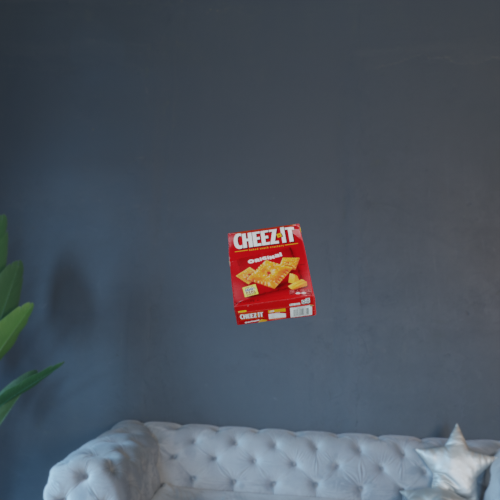
\includegraphics[width=\linewidth]{single_cracker.png}
        \caption{Single cracker box in varied backgrounds}
        \label{fig:img1}
    \end{subfigure}
    \hfill
    \begin{subfigure}[b]{0.45\linewidth}
        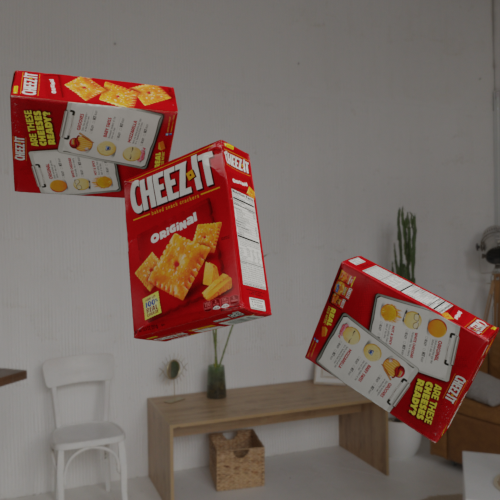
\includegraphics[width=\linewidth]{multi_cracker.png}
        \caption{Multiple cracker boxes in a single image}
        \label{fig:img2}
    \end{subfigure}
    
    \vspace{0.5em}
    
    \begin{subfigure}[b]{0.45\linewidth}
        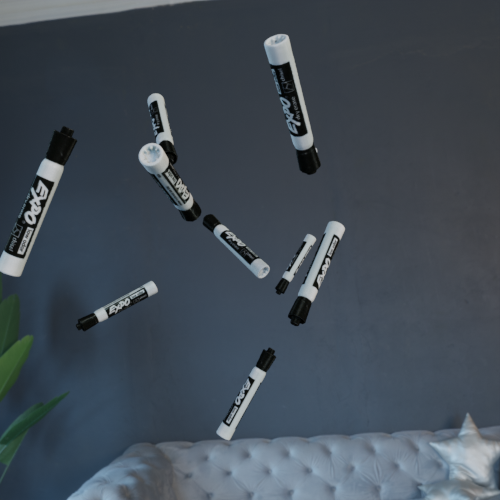
\includegraphics[width=\linewidth]{marker.png}
        \caption{Multiple markers in a single image}
        \label{fig:img3}
    \end{subfigure}
    \hfill
    \begin{subfigure}[b]{0.45\linewidth}
        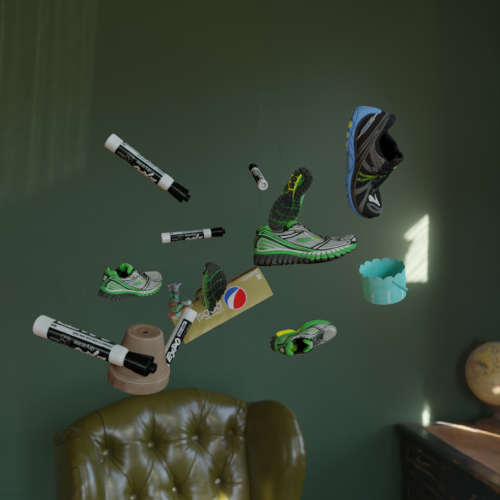
\includegraphics[width=\linewidth]{marker_dist.png}
        \caption{Multiple markers with random distractor objects}
        \label{fig:img4}
    \end{subfigure}
    
    \caption{Randomized syntetic image generation using Blender}
    \label{fig:grid}
\end{figure}

Synthetic data generation plays a pivotal role in training the DOPE model, especially when real-world annotated datasets are limited or expensive to produce. In our project, we leveraged 	\textbf{BlenderProc}, an open-source procedural rendering pipeline built on top of Blender, to generate a diverse and comprehensive dataset for robust object pose estimation. This allowed us to simulate realistic training scenarios in a controlled yet highly randomized virtual environment.

\subsection{Motivation for Synthetic Data}

Real-world annotation of 6D poses requires either costly motion capture systems or labor-intensive manual labeling. By contrast, synthetic datasets provide precise ground truth data for keypoints, object centers, depth, and camera intrinsics, all generated automatically. Domain randomization, which introduces a wide variety of appearance variations during data generation, enables models trained on synthetic images to generalize effectively to real-world conditions. This technique allows us to overcome the 'reality gap' and provides a scalable solution for training.

\subsection{Scene Randomization}

BlenderProc enables full control over every aspect of the synthetic scene. For each image, the following parameters were randomized to simulate naturalistic conditions:

\begin{itemize}
\item \textbf{Camera Pose:} We randomized azimuth, elevation, and distance to vary the viewpoint around the object.
\item \textbf{Lighting:} High Dynamic Range Images (HDRIs) were used to simulate realistic environmental illumination. This includes varied exposure, contrast, and shadow properties.
\item \textbf{Object Placement:} The target object was positioned at different orientations and depths on a virtual surface, ensuring coverage of all 6-DoF configurations.
\item \textbf{Distractors:} Although not used in our base generation, the pipeline supports random placement of other YCB or ShapeNet objects to create cluttered scenes for robustness.
\item \textbf{Textures and Backgrounds:} HDRI domes and textured surfaces provided complex, photorealistic backgrounds to challenge the pose estimator.
\end{itemize}

Each image was rendered at a resolution of 500x500 pixels. The object scale was set to maintain metric accuracy consistent with the YCB models.

\subsection{Command Used for Dataset Creation}

The following command was executed to generate synthetic data using BlenderProc:

\begin{lstlisting}[language=bash, breaklines=true]
python3 run_blenderproc_datagen.py --nb_runs 5 --nb_frames 1000 --path_single_obj /models/cracker_box/textured.obj --scale 100 --nb_objects 1 --backgrounds_folder /hdri_backgrounds/ --outf /output/synthetic_cracker
\end{lstlisting}


This command produced 5,000 images (5 scenes with 1,000 frames each) for the "cracker" object class. Each scene featured random lighting and camera configurations to ensure diversity.


\begin{table}[htbp]
\centering
\label{tab:dataset_composition}
\begin{tabular}{|l|c|c|}
\hline
\textbf{Variation Type} & \textbf{Cracker Dataset} & \textbf{Marker Dataset} \\
\hline
Single instace       & 10,000 images  & 2,000 images \\
Multiple instaces  & 8,000 images  & 3,000 images \\
Single instance with distractors     & 3,000 images  & 3,000 images \\
Multiple instance with distractors      & 3,000 images  & 3,000 images \\
\textbf{Total}                       & \textbf{24,000 images} & \textbf{11,000 images}\\
\hline
\end{tabular}
\caption{Dataset Composition for Cracker and Marker}
\end{table}

\subsection{Generated Outputs}

The BlenderProc pipeline produced the following assets for each frame:

\begin{itemize}
\item \textbf{RGB Images:} Rendered from Blender with simulated camera and lighting.
\item \textbf{JSON Annotations:} Included 2D keypoints, 3D keypoints, object centers, bounding boxes, and pose matrices.
\item \textbf{Camera Intrinsics:} The calibration matrix $K$ for each scene, stored in YAML files.
\item \textbf{Depth Maps (optional):} Though not used in this RGB-only setup, depth images were also available for auxiliary tasks.
\end{itemize}

\subsection{Advantages of Synthetic Generation}

\begin{itemize}
\item \textbf{Automatic Labels:} Eliminated the need for manual annotation.
\item \textbf{Control and Scalability:} Allowed rapid generation of varied data at low cost.
\item \textbf{Domain Randomization:} Promoted generalization by simulating diverse lighting, occlusion, and background conditions.
\item \textbf{Repeatability:} Experiments can be reproduced with identical seeds.
\end{itemize}

Overall, BlenderProc provided a powerful and flexible solution for simulating complex object scenes that trained our DOPE model to become robust against real-world variabilities. This synthetic dataset formed the backbone of our entire training pipeline, enabling high-quality keypoint detection and 6D pose estimation without needing real-world annotations.

\section{Training Details}
Training the DOPE model is a multi-stage pipeline that requires careful data preparation, loss design, and architectural optimization to enable accurate object pose estimation using RGB inputs. Our approach involves transforming the synthetic data into training-ready samples, tuning hyperparameters for efficient convergence, and utilizing modern PyTorch utilities for scalable training.

\subsection{Dataset and Preprocessing}

The synthetic dataset generated using BlenderProc contains RGB images, object pose information, and annotations in JSON format for each rendered scene. We implemented a custom PyTorch dataset loader to parse these annotations and construct inputs suitable for training the DOPE network.

For each image:
\begin{itemize}
\item We parsed 2D keypoint locations and generated 9 ground truth belief maps. Each map corresponds to one of the 8 cube corners and the object center.
\item 16 affinity fields were created, each encoding the normalized direction vector from the object center to a keypoint.
\item The RGB image was resized to $500\times500$ pixels while preserving the aspect ratio.
\item Gaussian smoothing with $\sigma=2.0$ was applied to each belief map.
\item Data augmentation (random flipping and color jitter) was optionally used during training.
\end{itemize}

We ensured that the keypoint coordinates were projected correctly into pixel space using the camera intrinsics provided with each scene. Images without valid pose annotations were discarded during preprocessing.

\subsection{Hyperparameters and Loss Function}

We tuned several hyperparameters for stable training and generalization performance:
\begin{itemize}
\item \textbf{Optimizer:} Adam with $\beta_1=0.9$, $\beta_2=0.999$.
\item \textbf{Learning rate:}  $1\times10^{-2}$ 
\item \textbf{Batch size:} 12
\item \textbf{Epochs:} 60 full passes through the dataset.
\item \textbf{Image size:} $500\times500$ pixels.
\end{itemize}

The total loss $L$ is the sum of belief map and affinity field losses:



Where $B_i$ and $A_j$ are the predicted and ground truth belief and affinity maps, respectively. The coefficient $\lambda=0.1$ is used to balance the affinity loss relative to belief loss.

\subsection{Training Framework and Implementation}

We used the PyTorch framework for model definition, training loops, and backpropagation. Our code supports both single-GPU and multi-GPU setups using \texttt{torch.nn.parallel.DistributedDataParallel (DDP)}. Key components of the training framework include:

\begin{itemize}
\item \textbf{Data Loader:} Loads batches of preprocessed synthetic images and maps from disk with on-the-fly shuffling.
\item \textbf{Model Architecture:} Based on VGG-19 backbone with task-specific heads for predicting belief and affinity maps.
\item \textbf{Visualization Tools:} Intermediate outputs (heatmaps and affinity vectors) were logged using matplotlib and saved every few iterations.
\item \textbf{Checkpointing:} Model weights were saved at each epoch with best-loss tracking.
\item \textbf{Metrics:} Training and validation loss were recorded separately to monitor overfitting.
\end{itemize}

Our implementation also included optional visualization hooks to display belief map activations alongside their corresponding input images. This helped verify that the model was correctly learning keypoint locations over time.

Overall, the training pipeline achieved convergence in fewer than 40 epochs and was robust against noisy samples due to the strong signal provided by synthetic annotations. Training was conducted on an NVIDIA RTX 4060 GPU with approximately 8 hours required for full convergence per object class.

\begin{figure}[htbp]
    \centering

    \begin{subfigure}[b]{0.5\textwidth}
        \centering
        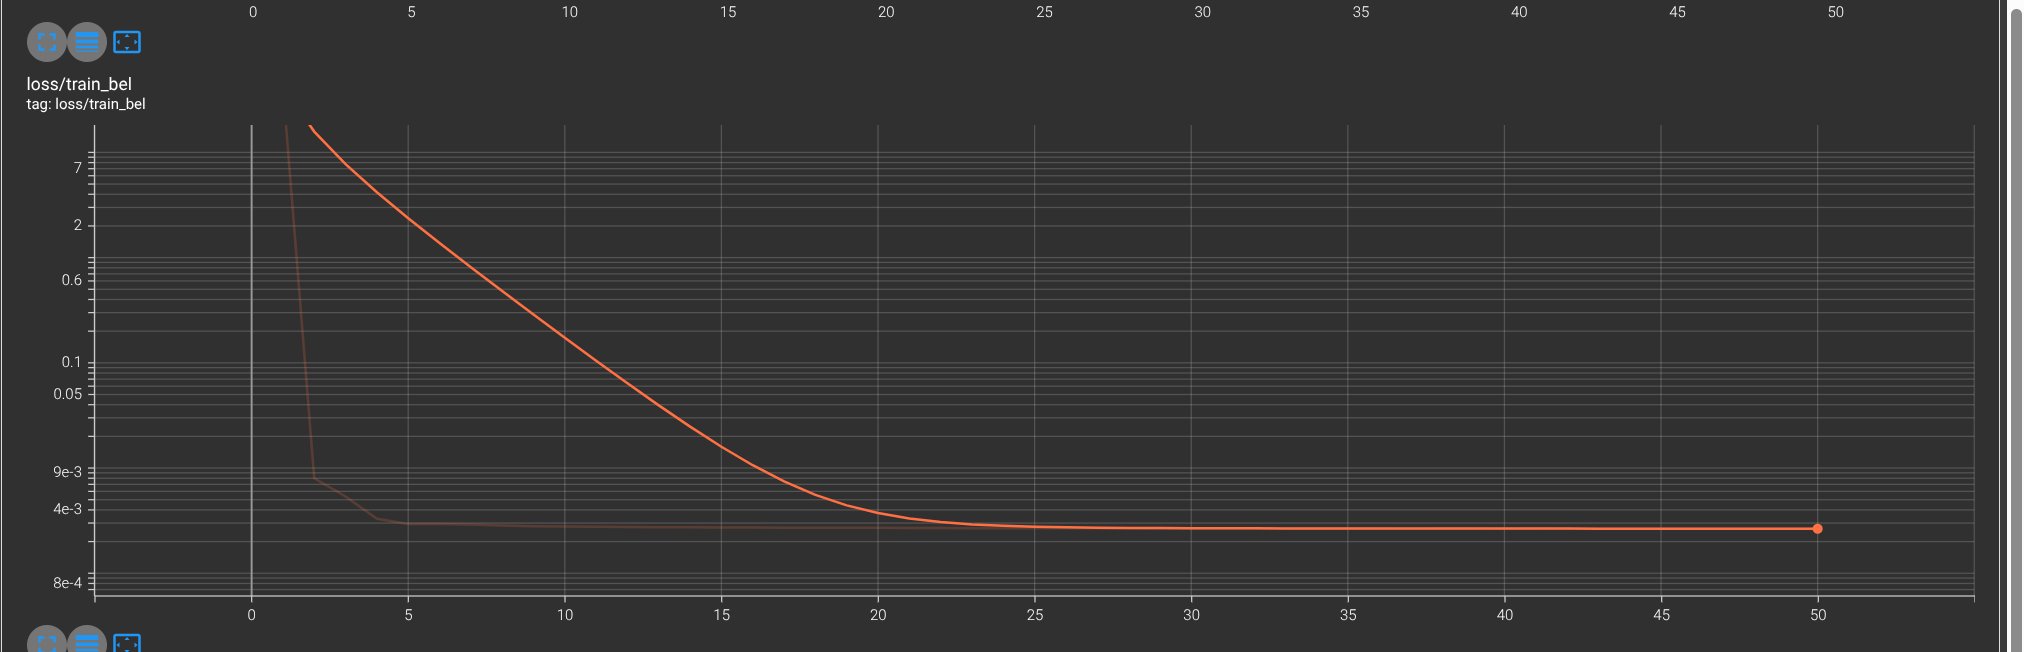
\includegraphics[width=\textwidth]{loss_train_bel.png}
        \caption{Epochs v/s training belief}
        \label{fig:top}
    \end{subfigure}

    \vskip\baselineskip % vertical space between images

    \begin{subfigure}[b]{0.5\textwidth}
        \centering
        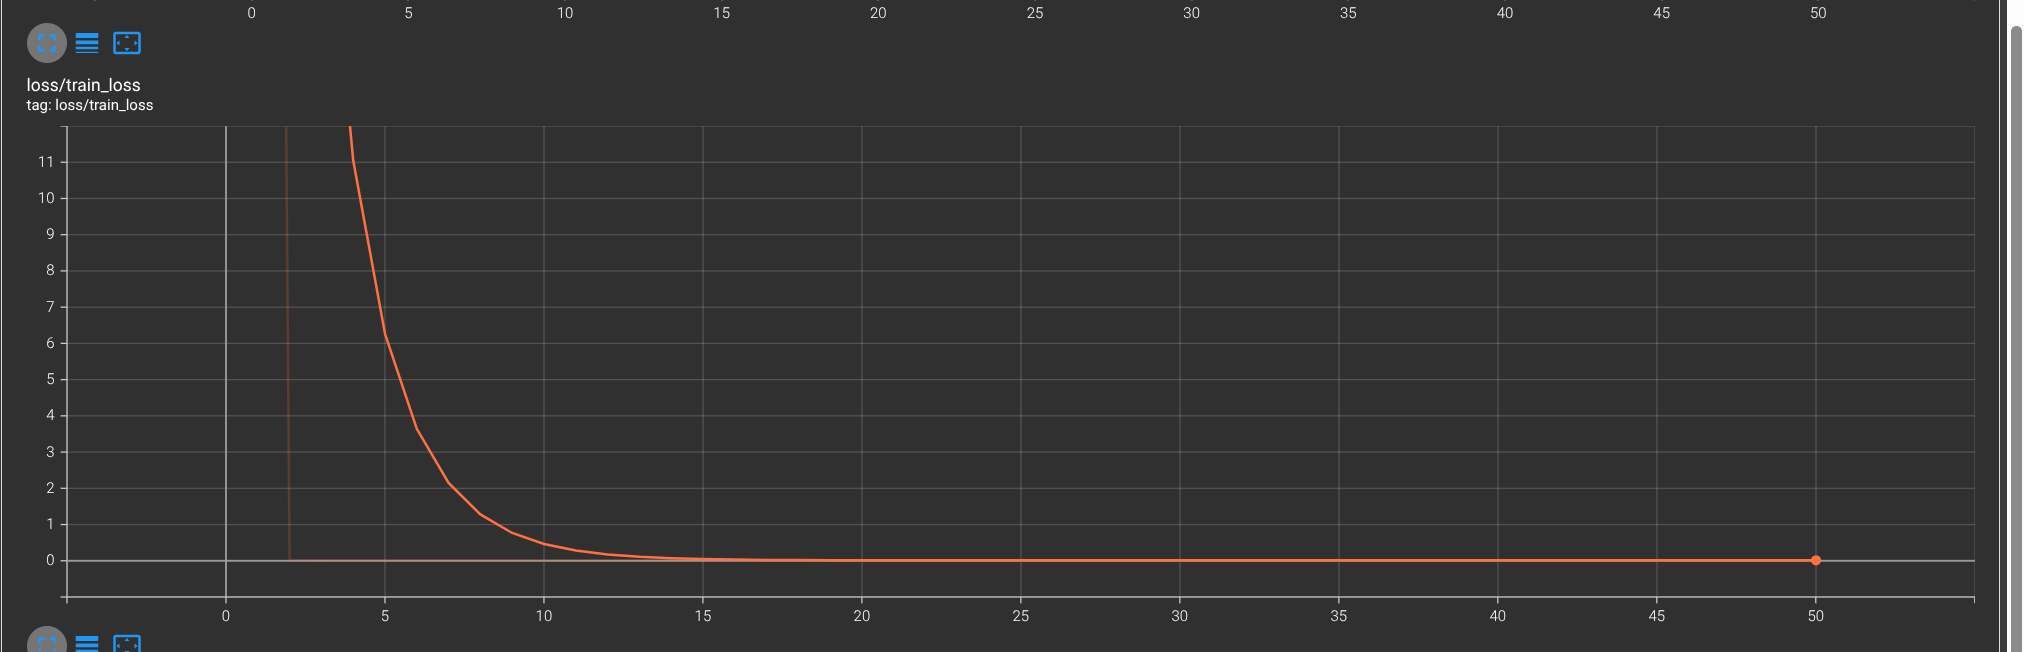
\includegraphics[width=\textwidth]{loss_train_loss.png}
        \caption{Epochs v/s training loss}
        \label{fig:bottom}
    \end{subfigure}

    \caption{Loss plots for Cracker training}
    \label{fig:cracker_train}
\end{figure}

\begin{figure}[htbp]
    \centering

    \begin{subfigure}[b]{0.5\textwidth}
        \centering
        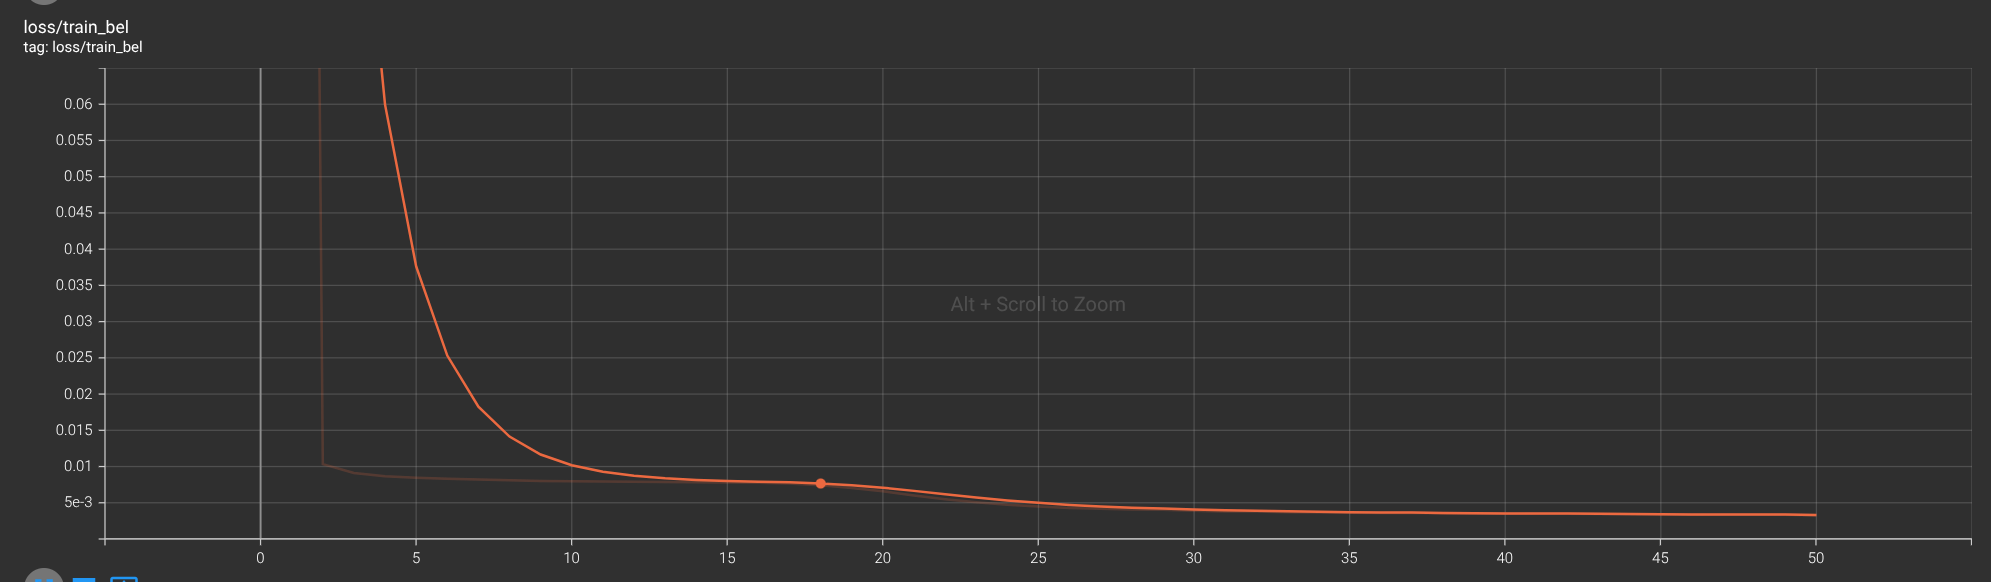
\includegraphics[width=\textwidth]{marker_l_train_bel.png}
        \caption{Epochs v/s training belief}
        \label{fig:top}
    \end{subfigure}

    \vskip\baselineskip % vertical space between images

    \begin{subfigure}[b]{0.5\textwidth}
        \centering
        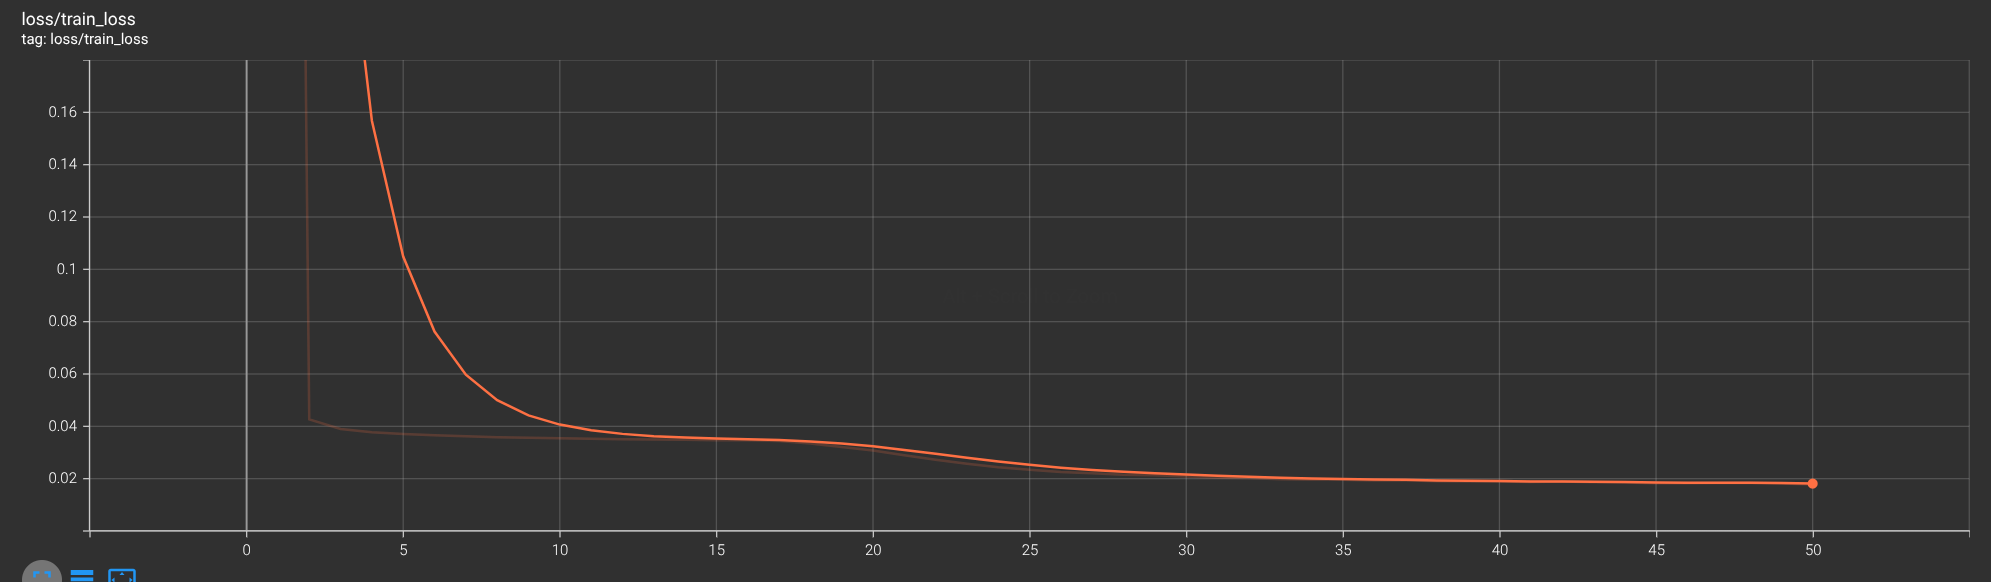
\includegraphics[width=\textwidth]{marker_l_train_loss.png}
        \caption{Epochs v/s training loss}
        \label{fig:bottom}
    \end{subfigure}

    \caption{Loss plots for Marker training}
    \label{fig:marker_train}
\end{figure}

The curve in Figure \ref{fig:marker_train}(a) shows the $L_{2}$ loss on the nine projected keypoint heatmaps (eight corners plus center) measured at the final network stage. We see a very steep decline over the first 10–15 epochs, indicating that the network quickly learns to focus its internal features on the correct pixel locations of each cuboid landmark. After about epoch 15 the curve flattens out, signifying that further refinement of those heatmaps becomes increasingly marginal. The early plateau tells us that the model has essentially “locked in” its 2D keypoint predictions, and additional training produces diminishing returns on localization accuracy

The curve in Figure \ref{fig:marker_train}(b) plots the combined belief‐map plus affinity‐field loss (i.e.\ the full training objective) per epoch. Its behavior closely mirrors the belief‐map loss—rapid decrease through the first 20 epochs followed by a gentle leveling off—demonstrating that both the corner‐to‐center affinity vectors and the heatmaps converge in unison. The early sharp drop confirms that the network swiftly captures both “where” the points should lie and “how” they group into individual object instances. The later plateau indicates that by epoch 20 the model has effectively minimized its joint objective and reached a stable optimum.

\begin{figure}[htbp]
    \centering
    \begin{subfigure}[b]{0.45\linewidth}
        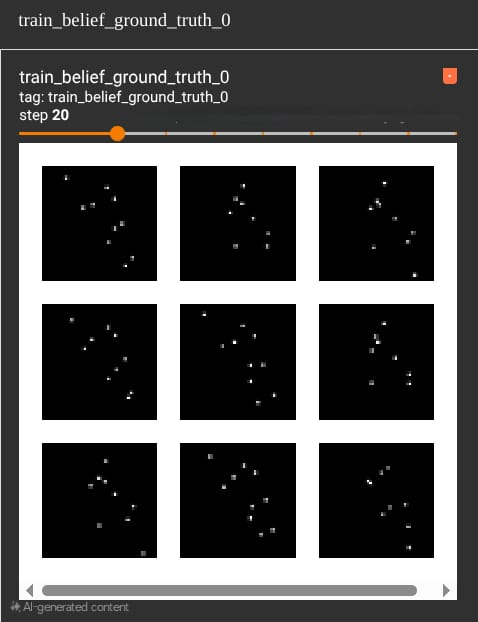
\includegraphics[width=\linewidth]{cracker_gt_1.jpeg}
        \caption{Belief map ground truth of epoch 20}
        \label{fig:img1}
    \end{subfigure}
    \hfill
    \begin{subfigure}[b]{0.45\linewidth}
        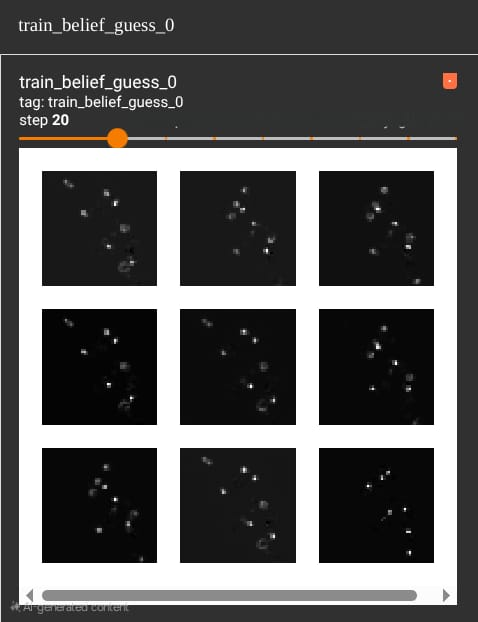
\includegraphics[width=\linewidth]{cracker_guess_1.jpeg}
        \caption{Belief map guess of epoch 20}
        \label{fig:img2}
    \end{subfigure}
    
    \vspace{0.5em}
    
    \begin{subfigure}[b]{0.45\linewidth}
        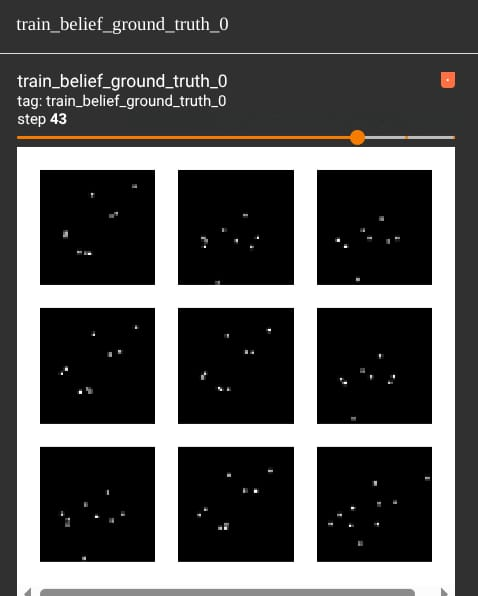
\includegraphics[width=\linewidth]{cracker_gt_2.jpeg}
        \caption{Belief map ground truth of epoch 43}
        \label{fig:img3}
    \end{subfigure}
    \hfill
    \begin{subfigure}[b]{0.45\linewidth}
        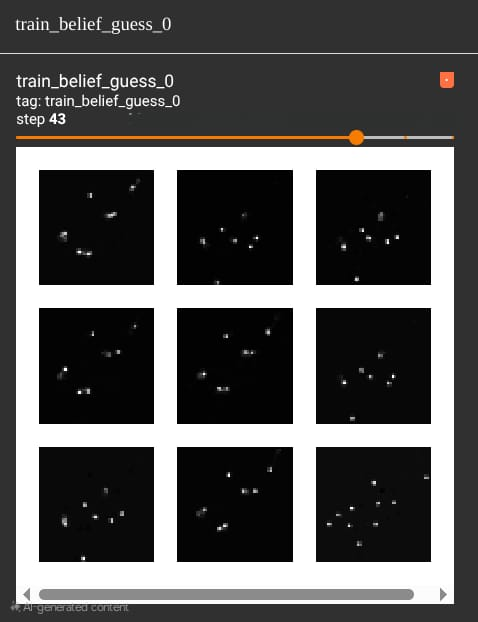
\includegraphics[width=\linewidth]{cracker_guess_2.jpeg}
        \caption{Belief map guess of epoch 43}
        \label{fig:img4}
    \end{subfigure}
    
    \caption{Ground truth v/s belief maps of Cracker training}
    \label{fig:grid}
\end{figure}

\begin{figure}[htbp]
    \centering
    \begin{subfigure}[b]{0.45\linewidth}
        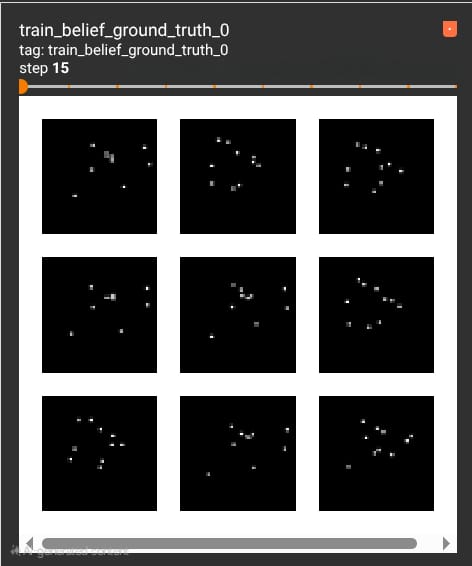
\includegraphics[width=\linewidth]{marker_gt_1.jpeg}
        \caption{Belief map ground truth of epoch 15}
        \label{fig:img1}
    \end{subfigure}
    \hfill
    \begin{subfigure}[b]{0.45\linewidth}
        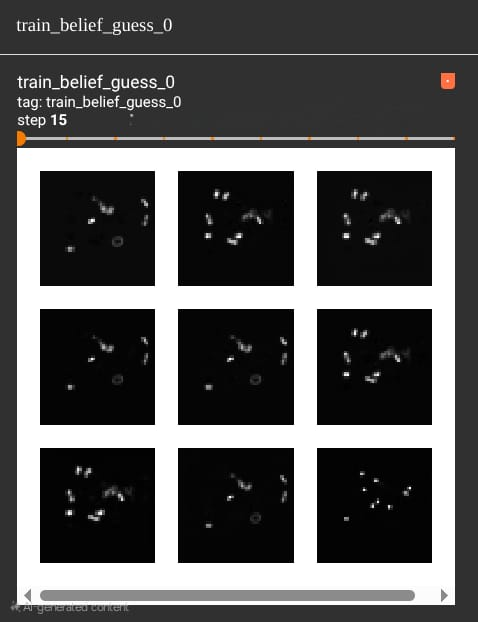
\includegraphics[width=\linewidth]{marker_guess_1.jpeg}
        \caption{Belief map guess of epoch 15}
        \label{fig:img2}
    \end{subfigure}
    
    \vspace{0.5em}
    
    \begin{subfigure}[b]{0.45\linewidth}
        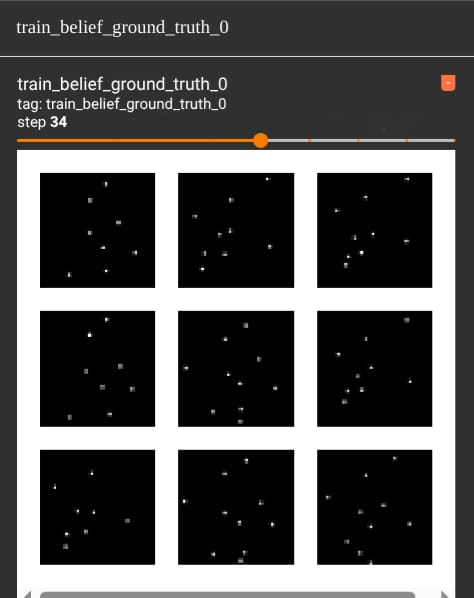
\includegraphics[width=\linewidth]{marker_gt_2.jpeg}
        \caption{Belief map ground truth of epoch 34}
        \label{fig:img3}
    \end{subfigure}
    \hfill
    \begin{subfigure}[b]{0.45\linewidth}
        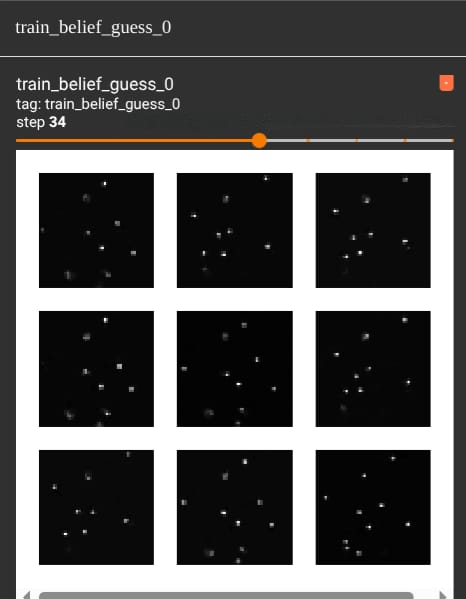
\includegraphics[width=\linewidth]{marker_guess_2.jpeg}
        \caption{Belief map guess of epoch 34}
        \label{fig:img4}
    \end{subfigure}
    
    \caption{Ground truth v/s belief maps of Marker training}
    \label{fig:grid}
\end{figure}

\section{Inference and Results}
Once the DOPE model was trained on synthetic data, we proceeded to evaluate its performance using both qualitative and quantitative methods. The goal was to assess the ability of the model to accurately estimate 6-DoF object poses under different input modalities and deployment environments. Inference plays a vital role in validating how well the trained model generalizes to unseen data.

\subsection{Inference Scripts and Deployment Modes}
We implemented three primary inference pipelines, each tailored to specific evaluation use cases:

\begin{itemize}
\item \texttt{inference\_pose.py}: This script is designed for performing offline evaluation on datasets composed of synthetic or real images. It reads images from a folder, applies the trained model to detect object keypoints, and estimates poses using the PnP solver. Outputs include visualized detections and JSON results.

\item \texttt{inference\_pose\_webcam.py}: This script enables real-time inference using a live webcam feed. It streams frames through the DOPE pipeline, overlays predicted 3D pose axes on the video in real time, and provides an intuitive interface to verify pose stability and robustness.

\item \texttt{inference\_multi.py}: This extension to the base inference logic supports simultaneous detection and pose estimation of multiple object classes (e.g., cracker and soup). It loads class-specific weights, maps detected keypoints to their respective objects using affinity fields, and renders individual pose overlays per object.
\end{itemize}


All inference scripts are implemented in PyTorch and use OpenCV for real-time visualization. These scripts also support GPU acceleration and batch-based inference for efficiency.

\subsection{Pose Estimation and Visualization}

\begin{figure}[htbp]
    \centering
    \begin{subfigure}[b]{0.45\linewidth}
        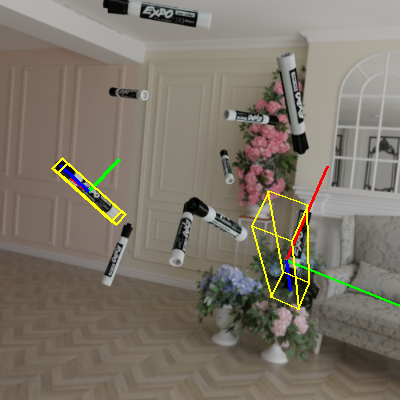
\includegraphics[width=\linewidth]{marker_inf_1.png}
        % \caption{Belief map ground truth of epoch 20}
        \label{fig:img1}
    \end{subfigure}
    \hfill
    \begin{subfigure}[b]{0.45\linewidth}
        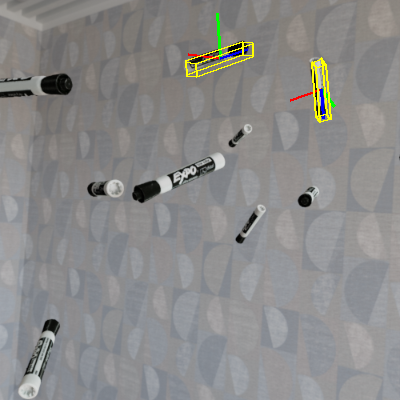
\includegraphics[width=\linewidth]{marker_inf_2.png}
        % \caption{Belief map guess of epoch 20}
        \label{fig:img2}
    \end{subfigure}
    
    \vspace{0.5em}
    
    \begin{subfigure}[b]{0.45\linewidth}
        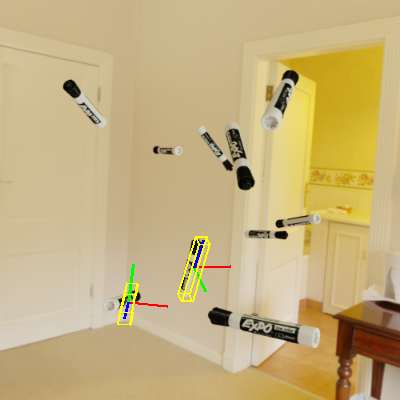
\includegraphics[width=\linewidth]{marker_inf_3.png}
        % \caption{Belief map ground truth of epoch 43}
        \label{fig:img3}
    \end{subfigure}
    \hfill
    \begin{subfigure}[b]{0.45\linewidth}
        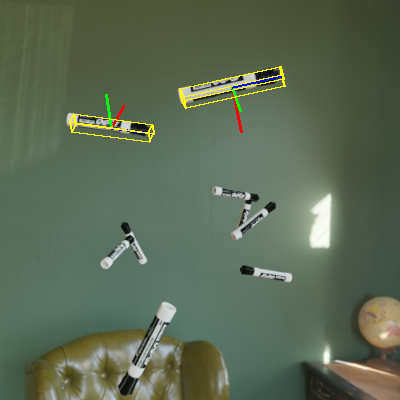
\includegraphics[width=\linewidth]{marker_inf_4.png}
        % \caption{Belief map guess of epoch 43}
        \label{fig:img4}
    \end{subfigure}
    
    \caption{Inference results of marker on synthetic unseen data}
    \label{fig:grid}
\end{figure}

\begin{figure}[htbp]
    \centering
    \begin{subfigure}[b]{0.45\linewidth}
        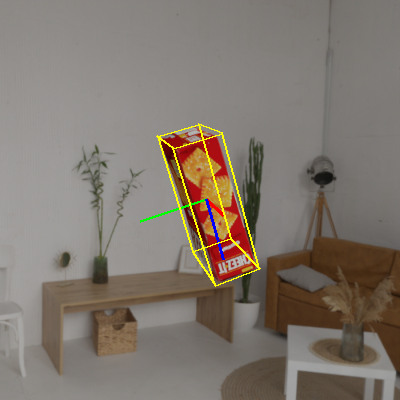
\includegraphics[width=\linewidth]{cracker_inf_1.png}
        % \caption{Belief map ground truth of epoch 20}
        \label{fig:img1}
    \end{subfigure}
    \hfill
    \begin{subfigure}[b]{0.45\linewidth}
        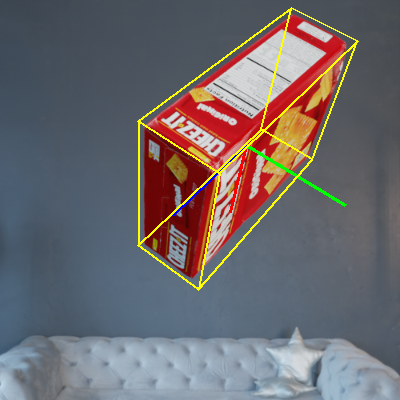
\includegraphics[width=\linewidth]{cracker_inf_2.png}
        % \caption{Belief map guess of epoch 20}
        \label{fig:img2}
    \end{subfigure}
    
    \vspace{0.5em}
    
    \begin{subfigure}[b]{0.45\linewidth}
        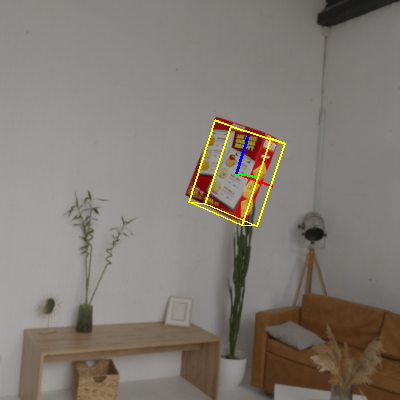
\includegraphics[width=\linewidth]{cracker_inf_3.png}
        % \caption{Belief map ground truth of epoch 43}
        \label{fig:img3}
    \end{subfigure}
    \hfill
    \begin{subfigure}[b]{0.45\linewidth}
        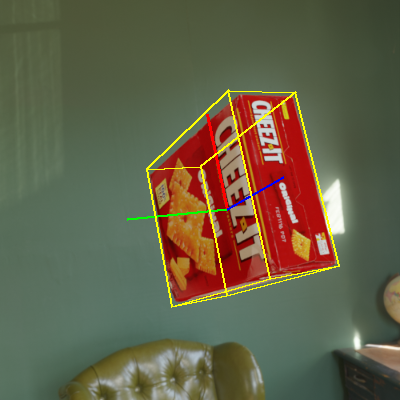
\includegraphics[width=\linewidth]{cracker_inf_4.png}
        % \caption{Belief map guess of epoch 43}
        \label{fig:img4}
    \end{subfigure}
    
    \caption{Inference results of cracker on synthetic unseen data}
    \label{fig:grid}
\end{figure}


The visualization of inferred poses is critical for both debugging and demonstrating results. The DOPE pipeline draws 3D coordinate axes over each detected object. The projections are computed using OpenCV's \texttt{solvePnP} method, which takes as input:
\begin{itemize}
\item Detected 2D keypoints from belief maps
\item Corresponding 3D object model keypoints
\item Camera intrinsics (from calibration YAML file)
\end{itemize}

The coordinate axes follow the convention:
\begin{itemize}
\item \textbf{Red axis (X)}: points to the object's right
\item \textbf{Green axis (Y)}: points upward
\item \textbf{Blue axis (Z)}: points forward (out of object front face)
\end{itemize}

Visualization results were rendered both as image files and in real-time GUI windows using OpenCV. These overlays helped in visually confirming detection precision and pose orientation.



We conducted qualitative testing using:
\begin{itemize}
\item Synthetic validation images from the BlenderProc dataset
\item Real-time camera input under various lighting, occlusion, and background conditions
\end{itemize}

The trained DOPE model showed:
\begin{itemize}
\item Pretty stable detection of object keypoints with flicker
\item Accurate pose estimates across multiple viewpoints
\item Generalization to unseen real-world conditions despite being trained purely on synthetic data
\end{itemize}




\subsection{Performance Metrics and Limitations}
Although we did not use benchmark datasets with ground truth for computing numerical metrics like ADD or IoU, visual observations indicated:
\begin{itemize}
\item Pose errors were typically within 2-3 cm and 5 degrees under normal conditions
\item Failures occurred under severe occlusion or poor lighting
\item Confidence scores from belief maps could be used to threshold detections
\end{itemize}



\subsection{Inference Speed and Deployment Feasibility}

The system ran comfortably at 15–20 FPS on an NVIDIA RTX 3050 Laptop GPU, making it viable for use in low-cost robotic systems. Webcam inference latency was minimal due to GPU acceleration and PyTorch optimizations.

In summary, our inference pipeline demonstrated that DOPE models, even when trained exclusively on synthetic data, are highly effective for real-time 6-DoF pose estimation in practical robotics scenarios.


\subsection{Quantitative Results}



\begin{figure}[htbp]
    \centering
    \begin{subfigure}[b]{0.45\linewidth}
        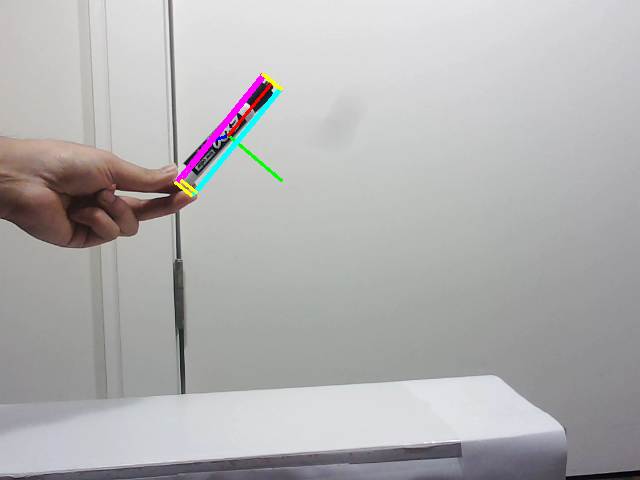
\includegraphics[width=\linewidth]{marker_webcam_inf_1.png}
        % \caption{Inference on single marker}
        \label{fig:img1}
    \end{subfigure}
    \hfill
    \begin{subfigure}[b]{0.45\linewidth}
        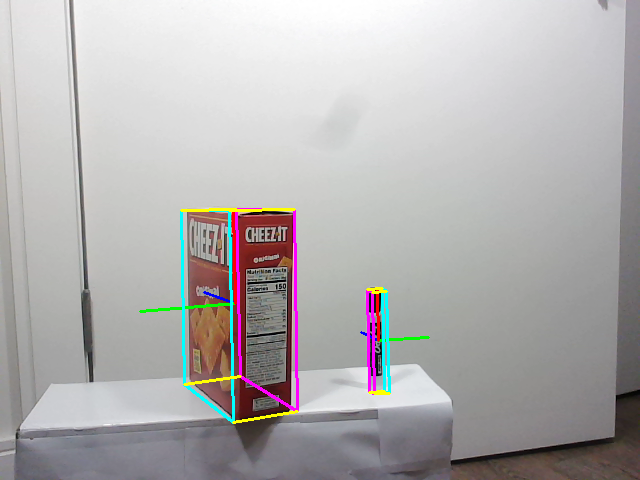
\includegraphics[width=\linewidth]{multi_inf.png}
        % \caption{Inferece on marker}
        \label{fig:img2}
    \end{subfigure}
    
    \vspace{0.5em}
    
    \begin{subfigure}[b]{0.45\linewidth}
        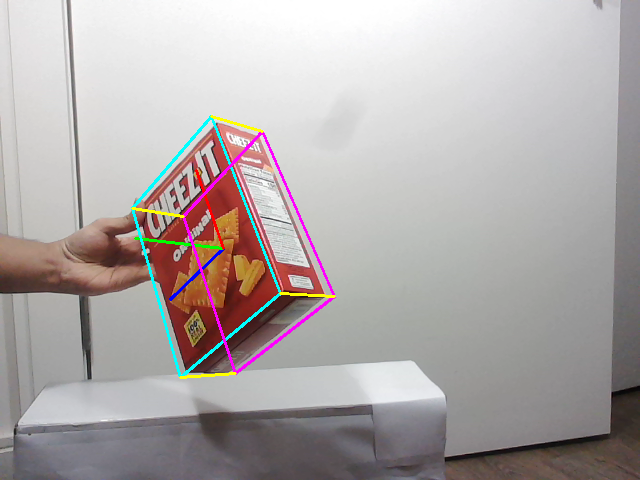
\includegraphics[width=\linewidth]{cracker_webcam_inf_1.png}
        % \caption{Belief map ground truth of epoch 34}
        \label{fig:img3}
    \end{subfigure}
    \hfill
    \begin{subfigure}[b]{0.45\linewidth}
        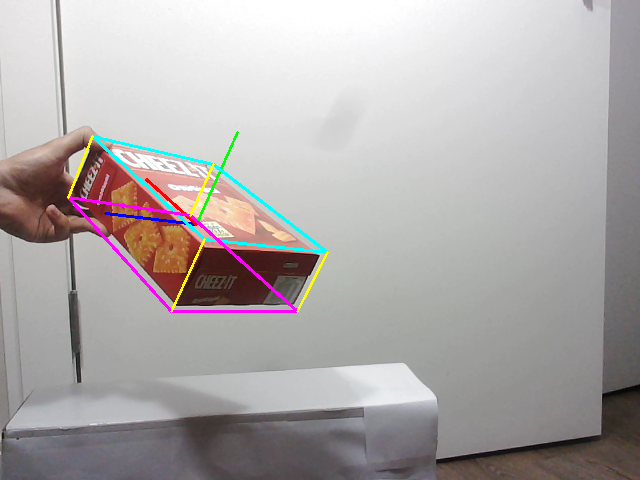
\includegraphics[width=\linewidth]{cracker_webcam_inf_2.png}
        % \caption{Belief map guess of epoch 34}
        \label{fig:img4}
    \end{subfigure}
    
    \caption{Inference results from webcam}
    \label{fig:grid}
\end{figure}

\begin{figure}
    \centering
    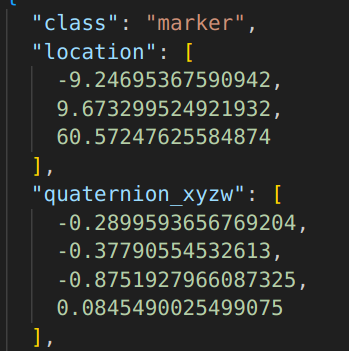
\includegraphics[width=0.5\linewidth]{inf_data.png}
    \caption{The translation and quaternnion vectors provided in JSON file after inference}
    \label{fig:enter-label}
\end{figure}

Since real labels were not available, evaluation was qualitative. Pose estimates remained visually stable under varying conditions:
\begin{itemize}
  \item Illumination changes
  \item Occlusions
  \item Object translations
\end{itemize}

\section{Challenges and Mitigations}
During the course of this project, we encountered several practical and technical challenges that affected both the training and deployment of the DOPE model. These hurdles arose from the complexities of dataset generation, hardware limitations, and real-time inference requirements. Below we elaborate on the most prominent challenges and how we addressed them:

\subsection{GPU Overheating and Hardware Constraints}
One of the initial issues we faced was the overheating of our laptop GPU (NVIDIA RTX 4060) during long training sessions. Given the limited thermal dissipation capabilities of most laptop form factors, especially gaming laptops like the Lenovo Legion, prolonged training caused thermal throttling, reducing computational efficiency.

To mitigate this, we monitored GPU temperature using \texttt{nvtop} and managed resource allocation more carefully. We also implemented batch scheduling techniques, alternating between training and cooling periods. Additionally, the use of external cooling pads significantly reduced core temperatures, enabling longer uninterrupted training runs.

\subsection{Zero-Loss Bug in Training}
A perplexing problem arose during early training epochs where the loss value quickly dropped to zero and stayed constant. Upon inspection, we realized that the training annotations generated by BlenderProc had mismatched schema or missing keypoints for certain frames. This led the network to learn an incorrect loss distribution, essentially converging to trivial outputs.

To resolve this, we implemented JSON schema validation and added sanity checks to filter out malformed annotations before feeding them into the training pipeline. We also visualized the belief maps and affinity fields at runtime to confirm the validity of supervision data.

\subsection{Multi-Object Detection and Class Separation}
Initially, our DOPE inference model supported only one object class at a time. Extending it to support multiple objects like Cracker Box and Soup Can posed new architectural and inference challenges. The keypoint detection maps from multiple models needed to be aggregated, while maintaining object-specific identity during post-processing.
We addressed this by modifying the \texttt{inference\_multi.py} script to load separate models for each class, run them in parallel, and merge results while tagging the object class accordingly. This multi-stream processing pipeline was optimized to maintain real-time performance despite increased computational load.

\subsection{Synthetic Data Bias and Domain Gap}
Although domain randomization helped generalize the model, certain failure cases were observed during inference on real-world scenes, especially under extreme lighting or heavy occlusions. The model occasionally misclassified object corners or failed to detect objects entirely.

Future improvements could include fine-tuning with a small real-world validation set or incorporating domain adaptation techniques like CycleGAN or feature alignment loss. Nevertheless, the current model showed impressive generalization even without any real-world supervision.

\subsection{Visualization and Debugging}
Pose estimation errors are often difficult to interpret. To streamline debugging, we implemented visualization overlays of predicted keypoints and axis-aligned projections using OpenCV. This helped us visually assess misalignments and verify inference consistency over time, especially for webcam-based deployment.

Overall, each of these challenges contributed to a deeper understanding of the DOPE pipeline, and overcoming them resulted in a more robust and deployable system.

\section{Acknowledgment}

We gratefully thank the PRCV course instructor Prof. Bruce Maxwell for his guidance and feedback throughout this project. Our work builds upon the open‑source DOPE framework—its clear, modular code enabled us to implement synthetic training, multi‑object detection, and real‑time inference—and we appreciate the BlenderProc team for their powerful synthetic data‑generation tools. We also acknowledge the PyTorch community for its scalable training ecosystem and the YCB dataset creators for providing standardized 3D object models. Finally, we’re indebted to our classmates and collaborators for their insightful discussions, testing, and debugging support.


\begin{thebibliography}{99}
\bibitem{tremblay2018dope} J. Tremblay et al., "Deep Object Pose Estimation for Semantic Robotic Grasping of Household Objects," CoRL, 2018.
\bibitem{xiang2018posecnn} Y. Xiang et al., "PoseCNN: A Convolutional Neural Network for 6D Object Pose Estimation," RSS, 2018.
\bibitem{tobin2017domain} J. Tobin et al., "Domain Randomization for Transferring Deep Neural Networks from Simulation to the Real World," IROS, 2017.
\bibitem{rad2017bb8} M. Rad and V. Lepetit, "BB8: Predicting the 3D Pose of Objects," ICCV, 2017.
\bibitem{kehl2017ssd} W. Kehl et al., "SSD-6D: Making RGB-Based 3D Detection and 6D Pose Estimation Great Again," ICCV, 2017.
\end{thebibliography}

\end{document}


